\documentclass[10pt,aspectratio=169,serif]{beamer}

\usepackage[fontset=none, scheme=plain]{ctex}
\IfFontExistsTF{Songti SC}{%
	\setCJKmainfont{Songti SC}[AutoFakeSlant=0.2]%
	\setCJKsansfont{Songti SC}[AutoFakeSlant=0.2]%
}{%
	\setCJKmainfont{FandolSong-Regular}[Extension=.otf,BoldFont=FandolSong-Bold,AutoFakeSlant=0.2]%
	\setCJKsansfont{FandolSong-Regular}[Extension=.otf,BoldFont=FandolSong-Bold]%
}
\usepackage{amsmath,amssymb,graphicx,tikz,booktabs,multicol,calligra}
\usepackage{pgfplots}
\pgfplotsset{compat=1.18}
\usepackage{tcolorbox}
\tcbuselibrary{skins}
\usepackage{XyygU}
\usepackage{caption}
\captionsetup[figure]{name=图,labelsep=period}

\usetikzlibrary{arrows.meta,positioning,calc}

% 公式间距
\setlength{\abovedisplayskip}{0pt plus 2pt minus 2pt}
\setlength{\belowdisplayskip}{0pt plus 2pt minus 2pt}

\title[习题1.3]{习题 1.3 集合的基本运算}
\subtitle{复习巩固 \& 综合运用 \& 拓广探索}
\author{}
\institute{}
\date{2026-10-16}

\begin{document}

\begin{frame}
  \titlepage
\end{frame}

% ========== A组 复习巩固 ==========
\begin{frame}[t]{A组：复习巩固}
本部分为教材第14页 习题1.3 复习巩固与综合运用，共6题。
\end{frame}

% ===== 第1题 =====
\begin{frame}[t]{第1题：区间型集合的交并}
\textbf{1.} 集合 $A = \{x \mid 2 \le x < 4\}$，$B = \{x \mid 3x - 7 \ge 8 - 2x\}$，求 $A \cup B$，$A \cap B$。
\end{frame}

\begin{frame}[t]{第1题 解答}
\begin{tcolorbox}[colback=orange!10,colframe=orange,title=\textbf{解}]
\textbf{先化简 $B$：} 解 $3x-7 \ge 8-2x$，即 $5x \ge 15$，得 $x \ge 3$，故
\[
B = \{x \mid x \ge 3\} = [3, +\infty).
\]
而 $A = [2, 4)$。

\textbf{求并集：} $A \cup B = [2, 4) \cup [3, +\infty) = [2, +\infty)$。

\textbf{求交集：} $A \cap B = [2, 4) \cap [3, +\infty) = [3, 4)$。
\end{tcolorbox}
\end{frame}

% ===== 第2题 =====
\begin{frame}[t]{第2题：多集合交并运算}
\textbf{2.} 设 $A = \{x \mid x \text{ 是小于 9 的正整数}\}$，$B = \{1, 2, 3\}$，$C = \{3, 4, 5, 6\}$。求 $A \cap B$，$A \cap C$，$A \cap (B \cup C)$，$A \cup (B \cap C)$。
\end{frame}

\begin{frame}[t]{第2题 解答}
\begin{tcolorbox}[colback=orange!10,colframe=orange,title=\textbf{解}]
\textbf{先化简 $A$：} 小于9的正整数为 $1,2,\dots,8$，故
\[
A = \{1,2,3,4,5,6,7,8\}.
\]

\textbf{逐项计算：}\\
$A \cap B = \{1,2,3\}$；\\
$A \cap C = \{3,4,5,6\}$；\\
$B \cup C = \{1,2,3,4,5,6\}$，故 $A \cap (B \cup C) = \{1,2,3,4,5,6\}$；\\
$B \cap C = \{3\}$，故 $A \cup (B \cap C) = A \cup \{3\} = \{1,2,3,4,5,6,7,8\}$。
\end{tcolorbox}
\end{frame}

% ===== 第3题 =====
\begin{frame}[t]{第3题：运动会集合的实际含义}
\textbf{3.} 学校开运动会，设 $A = \{x \mid x \text{ 是参加100 m跑的同学}\}$，$B = \{x \mid x \text{ 是参加200 m跑的同学}\}$，$C = \{x \mid x \text{ 是参加400 m跑的同学}\}$，学校规定，每个参加上述比赛的同学最多只能参加两项比赛，请你用集合的运算说明这项规定，并解释以下集合运算的含义：\\
(1) $A \cup B$；\qquad (2) $A \cap C$。
\end{frame}

\begin{frame}[t]{第3题 解答}
\begin{tcolorbox}[colback=orange!10,colframe=orange,title=\textbf{解}]
\textbf{学校规定：} 每个同学最多参加两项，即不能同时参加 $A,B,C$ 三项，故
\[
A \cap B \cap C = \varnothing.
\]

\textbf{(1) $A \cup B$：} 参加100 m跑\alert{或}参加200 m跑的同学，即参加100 m和200 m这两个项目之一的所有同学。

\textbf{(2) $A \cap C$：} 既参加100 m跑\alert{又}参加400 m跑的同学。
\end{tcolorbox}
\end{frame}

% ========== 综合运用 ==========
\begin{frame}[t]{B组：综合运用}
\end{frame}

% ===== 第4题 =====
\begin{frame}[t]{第4题：实数全集下的补集混合运算}
\textbf{4.} 已知集合 $A = \{x \mid 3 \le x < 7\}$，$B = \{x \mid 2 < x < 10\}$，求 $\complement_{\mathbf{R}}(A \cup B)$，$\complement_{\mathbf{R}}(A \cap B)$，$(\complement_{\mathbf{R}} A) \cap B$，$A \cup (\complement_{\mathbf{R}} B)$。
\end{frame}

\begin{frame}[t]{第4题 解答}
\begin{tcolorbox}[colback=orange!10,colframe=orange,title=\textbf{解}]
\textbf{先求交并：}
\[
A \cup B = (2, 10),\qquad A \cap B = [3, 7).
\]
\textbf{补集：}
\[
\complement_{\mathbf{R}}(A\cup B) = (-\infty, 2] \cup [10, +\infty);
\]
\[
\complement_{\mathbf{R}}(A\cap B) = (-\infty, 3) \cup [7, +\infty).
\]
\textbf{求 $(\complement_{\mathbf{R}} A)\cap B$：} $\complement_{\mathbf{R}}A = (-\infty,3)\cup[7,+\infty)$，与 $B=(2,10)$ 取交：
\[
(\complement_{\mathbf{R}}A)\cap B = (2,3) \cup [7,10).
\]
\textbf{求 $A\cup(\complement_{\mathbf{R}}B)$：} $\complement_{\mathbf{R}}B = (-\infty,2]\cup[10,+\infty)$，与 $A=[3,7)$ 取并：
\[
A\cup(\complement_{\mathbf{R}}B) = (-\infty,2]\cup[3,7)\cup[10,+\infty).
\]
\end{tcolorbox}
\end{frame}

% ===== 第5题 =====
\begin{frame}[t]{第5题：含参数方程解集的交并}
\textbf{5.} 设集合 $A = \{x \mid (x-3)(x-a)=0,\ a\in\mathbf{R}\}$，$B = \{x \mid (x-4)(x-1)=0\}$，求 $A \cup B$，$A \cap B$。
\end{frame}

\begin{frame}[t]{第5题 解答}
\begin{tcolorbox}[colback=orange!10,colframe=orange,title=\textbf{解}]
\textbf{化简 $B$：} $(x-4)(x-1)=0$ 得 $x=4$ 或 $x=1$，故 $B=\{1,4\}$。

\textbf{化简 $A$：} 方程 $(x-3)(x-a)=0$ 的根为 $x=3$ 和 $x=a$，需讨论 $a$。

\textbf{情况一：$a=3$（重根）} $A=\{3\}$，则
\[
A\cup B=\{1,3,4\},\quad A\cap B=\varnothing.
\]
\textbf{情况二：$a=1$} $A=\{1,3\}$，则
\[
A\cup B=\{1,3,4\},\quad A\cap B=\{1\}.
\]
\textbf{情况三：$a=4$} $A=\{3,4\}$，则
\[
A\cup B=\{1,3,4\},\quad A\cap B=\{4\}.
\]
\textbf{情况四：$a\neq 1,3,4$} $A=\{3,a\}$，则
\[
A\cup B=\{1,3,4,a\},\quad A\cap B=\varnothing.
\]
\end{tcolorbox}
\end{frame}

% ========== 拓广探索 ==========
\begin{frame}[t]{C组：拓广探索}
\end{frame}

% ===== 第6题 =====
\begin{frame}[t]{第6题：由补集反求集合}
\textbf{6.} 已知全集 $U = A \cup B = \{x \in \mathbf{N} \mid 0 \le x \le 10\}$，$A \cap (\complement_U B) = \{1, 3, 5, 7\}$，试求集合 $B$。
\end{frame}

\begin{frame}[t]{第6题 解答}
\begin{tcolorbox}[colback=orange!10,colframe=orange,title=\textbf{解}]
\textbf{先写出全集：}
\[
U = A\cup B = \{0,1,2,3,4,5,6,7,8,9,10\}.
\]

\textbf{分析 $A\cap(\complement_U B)$：} 该集合表示"属于 $A$ 但\alert{不属于} $B$"的元素，即
\[
A\cap(\complement_U B) = \{1,3,5,7\}.
\]
这说明 $1,3,5,7 \in A$ 且 $1,3,5,7 \notin B$。

\textbf{由于 $U = A\cup B$，除上述元素外，其余元素 $0,2,4,6,8,9,10$ 都必须属于 $B$（否则它们不在 $A\cup B$ 中）。}

\textbf{因此：}
\[
B = \{0,2,4,6,8,9,10\}.
\]
\vspace{0.5em}
\small（验证：$\complement_U B = \{1,3,5,7\}$，而 $A$ 至少含 $\{1,3,5,7\}$ 且与 $B$ 并为全集）
\end{tcolorbox}
\end{frame}

\begin{frame}[t]{第6题 配图：Venn图分析}
\begin{center}
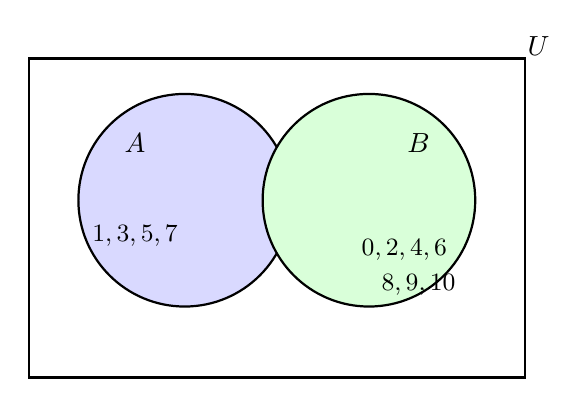
\begin{tikzpicture}[scale=0.9]
% 全集矩形
\draw[thick] (0,0) rectangle (7,4.5);
\node[above right] at (6.9,4.4) {$U$};

% A圆
\draw[thick,fill=blue!15] (2.2,2.5) circle (1.5);
\node at (1.5,3.3) {$A$};
\node[font=\small] at (1.5,2.0) {$1,3,5,7$};

% B圆
\draw[thick,fill=green!15] (4.8,2.5) circle (1.5);
\node at (5.5,3.3) {$B$};
\node[font=\small] at (5.3,1.8) {$0,2,4,6$};
\node[font=\small] at (5.5,1.3) {$8,9,10$};
\end{tikzpicture}
\end{center}
\vspace{-1em}
\begin{center}
\small{$A\cap(\complement_U B)=\{1,3,5,7\}$（A中不属于B的部分）}
\end{center}
\end{frame}

\begin{frame}[c]
  \begin{center}
    {\Huge\calligra Thanks!}
  \end{center}
\end{frame}

\end{document}
